\section{Performance Evaluation and Analysis}


The performance analysis section of this paper aims to measure and evaluate the power consumption, latency, and memory usage of the algorithms employed in the proposed scheme.

To measure the performance of our proposed solution, we prepared six case scenarios, which were categorized into two groups. The first group of three cases measured the performance from an algorithm perspective, while the second group of three cases measured the performance from a running application perspective.


\textit{Case 1: AES-GCM} - For this case, we use the AES-GCM encryption function to pass a plain text message and received encrypted and authenticated cipher text. 

\textit{Case 2: ASCON} - 
Unlike Case 1, the ASCON encryption function is employed to encrypt the message in this scenario.

\textit{Case 3: No encryption} - This case scenario was used as a baseline reference for the other two cases. In this case, we called a function that has a similar signature to the encryption function calls we used for ASCON and AES-GCM. However, the underlying function did not perform any operation other than copying values from one memory to another. The implementation code for this case can be seen in the following code list.

\begin{lstlisting}[style=CStyle]
int crypto_aead_encrypt(
      unsigned char *c,unsigned long long *clen,
      const unsigned char *m,unsigned long long mlen,
      const unsigned char *ad,unsigned long long adlen,
      const unsigned char *nsec,
      const unsigned char *npub,
      const unsigned char *k
      )
{
  *clen = mlen + CRYPTO_ABYTES;
  memcpy(c, m, mlen);
  memset(c + mlen, 0, CRYPTO_ABYTES);

  return 0;
}

int crypto_aead_decrypt(
  unsigned char *m, unsigned long long *mlen,
  unsigned char *nsec,
  const unsigned char *c, unsigned long long clen,
  const unsigned char *ad, unsigned long long adlen,
  const unsigned char *npub,
  const unsigned char *k
)
{
  unsigned long long len = *mlen = clen - CRYPTO_ABYTES;
  memcpy(m, c, len);

  return 0;
} 
\end{lstlisting}


\subsection{Speed - Running Time}
% execution time 
% 
In the Arduino ESP-IDF framework, we measure the execution time of a function using the built-in functions provided by the framework. The \texttt{esp\_timer\_get\_time()} function is used to retrieve the current time in microseconds since the underlying device boot. By capturing the start time before executing the function and the end time after the function completes, we calculate the execution time by subtracting the start time from the end time.

Our experimental setup involves three distinct case scenarios. Firstly, we measure the execution time when the application runs without any encryption algorithm. Then, we measure the execution time when the messages are encrypted using ASCON and AES algorithms. Note that we measure the performance of the proposed solution from two perspectives; 1) From the time required to run the encryption algorithm within the application program and 2) from the perspective of measuring the total time required to process message and send it to the digital twin (Cloud). Both case scenarios are shown in figure Fig \ref{Fig:time-scheme} and Fig \ref{Fig:time-algorithm}. 

To obtain accurate measurements, we allow our programs to run 1000 function calls sending data after encryption for each case scenario. We then calculate the average execution time using a Python script that processes the dump file we collected from the device.

As it can be seen from Figure \ref{Fig:time-algorithm} ASCON's execution time is lower than AES-GCM. However, Figure \ref{Fig:time-scheme} shows that our proposed solution performs well when the underlying encryption algorithm is AES-GCM.[I can't figure out the reason...]

\begin{figure}[H]
        % \centering
        \begin{subfigure}[c]{0.48\linewidth}
            \resizebox{\linewidth}{!}{
                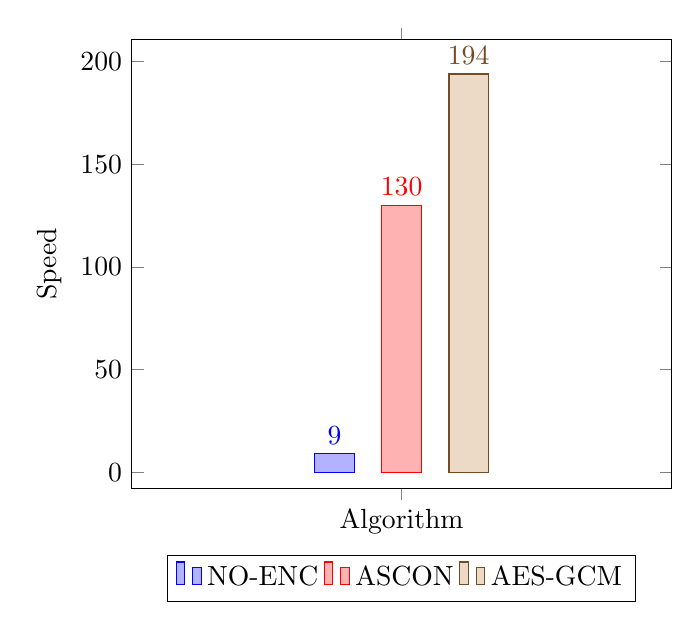
\begin{tikzpicture}
                    \begin{axis}[
                        ybar = 10pt,
                        enlargelimits=0.09,
                        legend style={at={(0.5,-0.15)},
                        anchor=north,legend columns=-1},
                        ylabel={Speed},
                        symbolic x coords={Algorithm, Scheme},
                        xtick=data,
                        nodes near coords,
                        nodes near coords align={vertical},
                        bar width = 0.5cm,
                        ]
                        \addplot coordinates {(Algorithm,9)};
                        \addplot coordinates {(Algorithm,130)};
                        \addplot coordinates {(Algorithm,194)};
                        % \addplot coordinates {(Algorithm,2)};
                         
                        \legend{NO-ENC, ASCON, AES-GCM}
                    \end{axis}
                \end{tikzpicture}
            }
        \caption{Speed From The Algorithm Execution Perspective.}
        \label{Fig:time-algorithm}
    \end{subfigure}%
    \begin{subfigure}[c]{0.48\linewidth}
        \resizebox{\linewidth}{!}{
            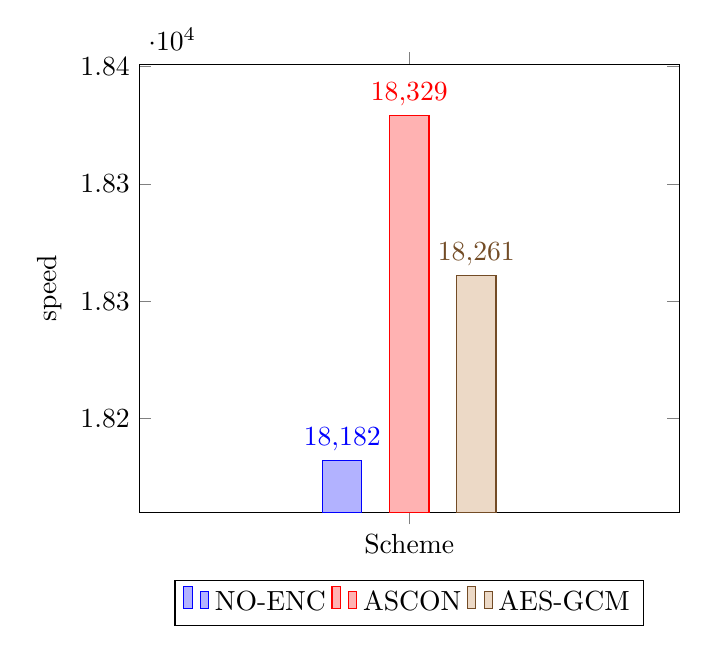
\begin{tikzpicture}
                \begin{axis}[
                    ybar = 10pt,
                    enlargelimits=0.15,
                    legend style={at={(0.5,-0.15)},
                    anchor=north,legend columns=-1},
                    ylabel={speed},
                    symbolic x coords={Scheme},
                    xtick=data,
                    nodes near coords,
                    nodes near coords align={vertical},
                    bar width = 0.5cm,
                    ]
                    \addplot coordinates {(Scheme,18182)};
                    \addplot coordinates {(Scheme,18329)};
                    \addplot coordinates {(Scheme,18261)};
                    % \addplot coordinates {(Algorithm,2)};
                     
                    \legend{NO-ENC, ASCON, AES-GCM}
                \end{axis}
            \end{tikzpicture}
            }
    \caption{Speed From The Scheme (Application) Perspective.}
    \label{Fig:time-scheme}
\end{subfigure}
\caption{Sample of how to use subfigures.}
\label{Fig:Theo_SFDev}
\end{figure}

\subsubsection*{Throughput and Cycle Byte Ratio}

Throughput is a performance indicator of a system that measures the number of bytes processed per unit of time (typically seconds). It is a measure of how efficiently a system can process data. The more bytes that are processed per unit of time, the better the system performs. Throughput is typically measured in bytes per second (Bps) or kilobytes per second (Kbps).

The Cycle Byte Ratio is another performance metric that measures the number of CPU cycles needed to process a single byte. Table \ref{tbl:cycle-count} presents the cycle counts for different scenarios: 1) without employing any encryption algorithm, 2) utilizing the ASCON encryption algorithm, and 3) employing the AES-GCM encryption algorithm.


\begin{table}[H]
    \centering
    \caption{Cycle Count For 3 Cases: No-Encryption, ASCON, AES-GCM }
    \label{tbl:cycle-count}
    \resizebox{\textwidth}{!}
    {
        \begin{tabular}{l | a | b | a}
        \hline
        \rowcolor{LightCyan}
        \mc{1}{}  & \mc{1}{No-Encryption}  & \mc{1}{ASCON} & \mc{1}{AES-GCM}\\
        \hline
        Cycle Count & 2009 & 36811  &  49956\\
        Byte Processed & 32  & 32 &  32\\ 
        CPU Freq MHz & 240 & 240 &  240\\ 
        Cycle per Byte &  64.28 & 1094.68 &  31517.90\\ 
        Time Elapsed $\mu$s & 8.57  & 145.95 &  202.38\\ 
        Throughput B/$\mu$s & 3.73  & 0.219 &  0.158\\ 
        \hline
        \end{tabular} 
        }
\end{table}

\begin{equation}
\text{Throughput} = \frac{\text{Byte processed}}{\text{Total Time}} \quad \text{Cycle Byte} = \frac{\text{Cycle Count}}{\text{Byte processed}}
\end{equation}

The total time taken by the CPU to perform an operation can be derived using cycle count and the CPU clock frequency. The total time taken by the operation is equal to the cycle count multiplied by the CPU clock frequency. 

To calculate the throughput and the cycle byte ratio for each algorithm in our proposed solution, we use 64 bytes of data as input. The summarized statical data is provided in Figure \ref{fig:per-cb}

\begin{equation}
\text{Total Time} = \frac{\text{Cycle Count}}{\text{CPU frequency in Mhz/Khz}}
\end{equation}

In this experiment, while we use \texttt{$xthal\_get\_ccount()$} from esp32/ck.h library to get the cycle count at a given time, we use \texttt{$getCpuFrequencyMhz()$} function to get the current set CPU frequency of the device fro esp32-hal-cpu.c source file.  

We calculated the throughput and cycle byte ratio of each algorithm in the proposed solution processing 16 bytes of message and 16 bytes of associated data, using equation (4.1). The results are shown in Figures \ref{fig:put} and \ref{fig:ccb-ratio}.


\begin{figure}[H]
        % \centering
        \begin{subfigure}[c]{0.48\linewidth}
            \resizebox{\linewidth}{!}{
                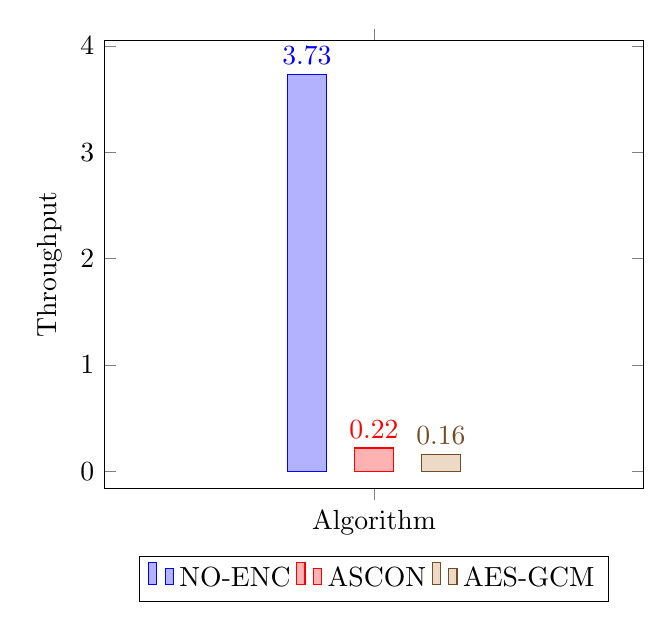
\begin{tikzpicture}
                    \begin{axis}[
                        ybar = 10pt,
                        enlargelimits=0.09,
                        legend style={at={(0.5,-0.15)},
                        anchor=north,legend columns=-1},
                        ylabel={Throughput},
                        symbolic x coords={Algorithm},
                        xtick=data,
                        nodes near coords,
                        nodes near coords align={vertical},
                        bar width = 0.5cm,
                        ]
                        \addplot coordinates {(Algorithm,3.73)};
                        \addplot coordinates {(Algorithm,0.219)};
                        \addplot coordinates {(Algorithm,0.158)};
                         
                        \legend{NO-ENC, ASCON, AES-GCM}
                    \end{axis}
                \end{tikzpicture}
            }
        \caption{Throughput of the algorithms.}
        \label{Fig:put}
    \end{subfigure}%
    \begin{subfigure}[c]{0.48\linewidth}
        \resizebox{\linewidth}{!}{
            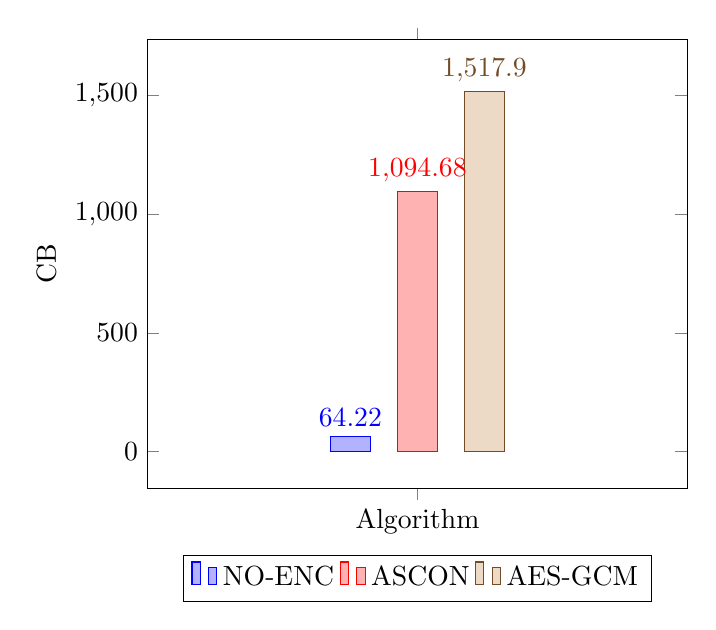
\begin{tikzpicture}
                \begin{axis}[
                    ybar = 10pt,
                    enlargelimits=0.15,
                    legend style={at={(0.5,-0.15)},
                    anchor=north,legend columns=-1},
                    ylabel={C\\B},
                    symbolic x coords={Algorithm},
                    xtick=data,
                    nodes near coords,
                    nodes near coords align={vertical},
                    bar width = 0.5cm,
                    ]
                    \addplot coordinates {(Algorithm,64.218)};
                    \addplot coordinates {(Algorithm,1094.68)};
                    \addplot coordinates {(Algorithm,1517.90)};
                    % \addplot coordinates {(Algorithm,2)};
                     
                    \legend{NO-ENC, ASCON, AES-GCM}
                \end{axis}
            \end{tikzpicture}
            }
    \caption{Cycle per Byte ratio.}
    \label{Fig:ccb-ratio}
\end{subfigure}
\caption{Throughput and cycle per byte ratio of each algorithms.}
\label{Fig:Theo_SFDev}
\end{figure}


% ****************************************************************************************
\subsection{Static and Dynamic Memory Footprint }
% show the ram and flash memory of embeded progrma 
Analyzing and measuring the memory usage of embedded programs is vital, especially when the device has memory constraints. In this section, we will discuss the static and dynamic memory usage of our proposed solution. Throughout our measurement,  compared three implementations scenarios:
\begin{itemize}
    \item No encryption,
    \item Encryption using ASCON, and
    \item Encryption using AES-GCM
\end{itemize}



\begin{figure}[H]
    \centering
    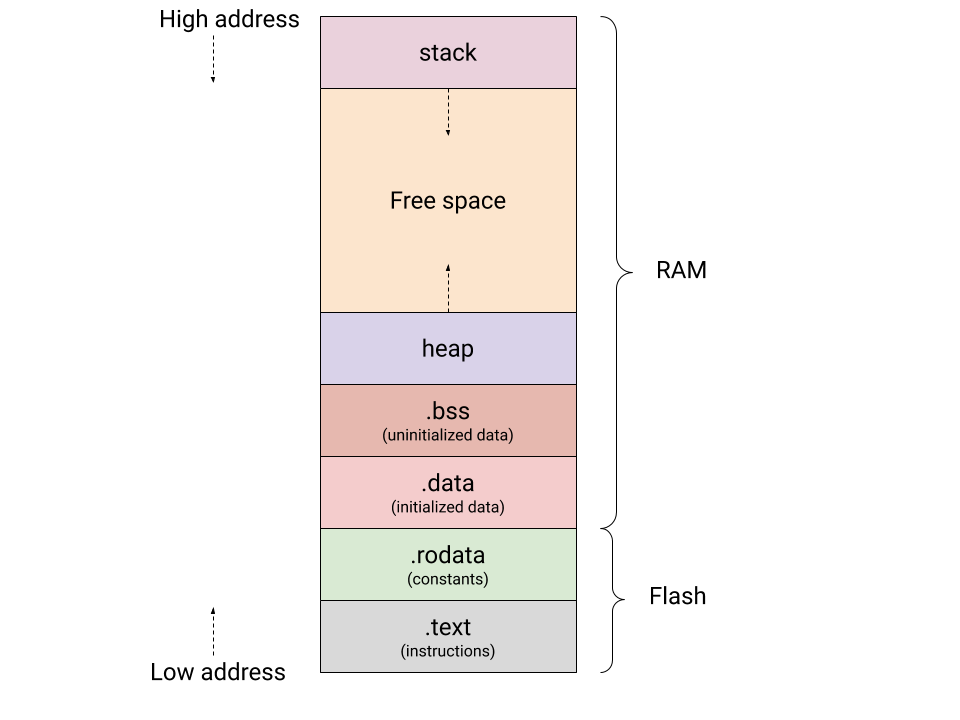
\includegraphics[width=\linewidth]{images/fp/memory-analysis.png}
    \caption{Memory Map of Embedded Programming \cite{alcarazDigitalTwinComprehensive2022}}
    \label{fig:memory-map}
\end{figure}

Figure \ref{fig:memory-map} depicts the general memory map of embedded programming. The flash part of the memory that includes the .rodata and .text section contains the code resulting from compiling and building the source program. This section contains static codes and requires a fixed memory size. Whereas, the RAM section of the memory is responsible for containing a few sections for statically generated codes and the majority one for handling dynamic memory management such as stack and heap allocation.


In our analysis of the dynamic memory usage for our implementation of the proposed solution, we focused only on the RAM section. However, when assessing the static memory usage (code size), we examined both the RAM and Flash sections. This approach was necessary as both sections contribute to the overall code size. 

\subsubsection{Static Memory Usage - Code size}
% Provide a table 
% Draw a graph 

The static code size measurement was conducted to compare the code size requirements of three different implementation scenarios: No-Encryption, ASCON, and AES-GCM. The goal was to assess the impact of these implementations on resource-constrained devices in terms of memory usage.

Table \ref{tbl:ins-codesize} provides a summary of the code size measurements for each scenario. In the No-Encryption scenario, no additional code was required beyond the base program, resulting in minimal memory usage. Our implementation based on ASCON introduced a slight increase in code size. Approximately 1 KB of additional memory was needed in both RAM and Flash compared to the No-Encryption scenario. On the other hand, AES-GCM demonstrated slightly higher code size requirements. The implementation demanded approximately 8 KB more RAM and 5.6 KB more Flash memory compared to the No-Encryption case.


\begin{table}[H]
    \centering
    \caption{Code Size: No-Encryption, ASCON, AES-GCM }
    \label{tbl:ins-codesize}
    \resizebox{\textwidth}{!}
    {
        \begin{tabular}{l | a | b | a}
        \hline
        \rowcolor{LightCyan}
        \mc{1}{}  & \mc{1}{No-Encryption}  & \mc{1}{ASCON} & \mc{1}{AES-GCM}\\
        \hline
        Ram \/KB & 59.3 & 59.3  &  68\\
        Flash & 766.5  & 767.7 &  772.1\\ 
        Total & 825.8 & 827 &  840.1\\ 
        % Cycle per Byte &  64.28 & 1094.68 &  31517.90\\ 
        % Time Elapsed $\mu$s & 8.57  & 145.95 &  202.38\\ 
        % Throughput B/$\mu$s & 3.73  & 0.219 &  0.158\\ 
        \hline
        \end{tabular} 
        }
\end{table}

\begin{figure}[H]
    \centering
    \caption{Static Code Size of The Scheme For 3 Scenarios(No-Encryption, ASCON, AES-GCM}
    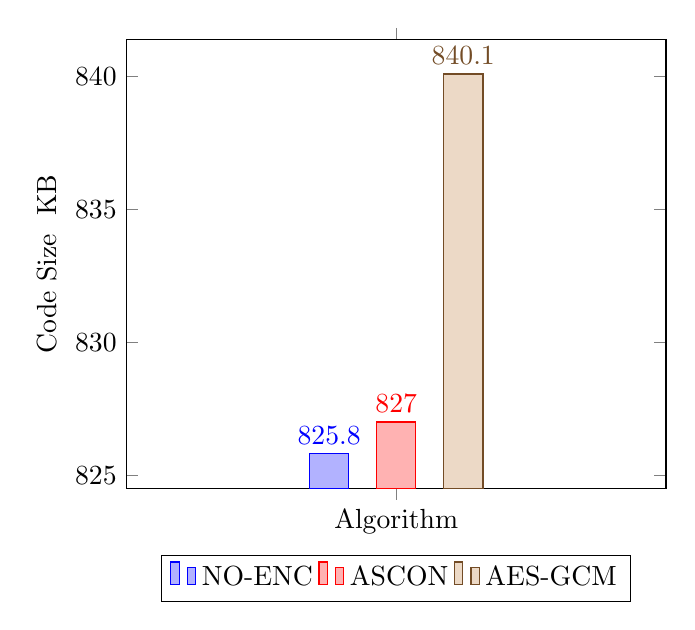
\begin{tikzpicture}
        \begin{axis}[
            ybar = 10pt,
            enlargelimits=0.09,
            legend style={at={(0.5,-0.15)},
            anchor=north,legend columns=-1},
            ylabel={Code Size \/ KB},
            symbolic x coords={Algorithm},
            xtick=data,
            nodes near coords,
            nodes near coords align={vertical},
            bar width = 0.5cm,
            ]
            \addplot coordinates {(Algorithm,825.8)};
            \addplot coordinates {(Algorithm,827)};
            \addplot coordinates {(Algorithm,840.1)};
             
            \legend{NO-ENC, ASCON, AES-GCM}
        \end{axis}
    \end{tikzpicture}    
\label{Fig:codesize}
\end{figure}

\subsubsection{Dynamic RAM Usage}

% I will explain the techniques I used to capture the memory usage
% The challenge of measuring the memory heap 
% Explain or provide an analysis of memory for each case 

Measuring the dynamic RAM usage of each algorithm is not as easy as measuring static memory usage. The heap and stack are two types of dynamic memory, making it challenging to keep track of their usage as they are allocated and freed during function calls and returns. One effective technique recommended by NIST is to overwrite the memory with known values before running the program and keeping track of the memory cells that are overwritten by the program [ref]. However, due to the complexity of setting it up,  we decided to employ alternative techniques to approximate the dynamic memory usage of each algorithm described as follows.



In our device (ESP32), we discovered that the initially allocated memory for handling heap and stack allocation is 327,680 Bytes. Having this in mind, we tracke the minimum heap size ever available, utilising the system call \textit{esp\_get\_minimum\_free\_heap\_size}. Our program was executed for 1000 iterations calling the encryption function for each implementation, allowing us to obtain a snapshot of the free memory available between the stack and heap 1000 times. By calculating the difference between the total allocated dynamic memory and the minimum heap size recorded, we were able to approximate the memory footprint of each implementation.

Furthermore, we employed the baseline implementation, which does not incorporate an encryption/decryption algorithm, as a benchmark to estimate the dynamic memory usage overhead added by ASCON and AES-GCM algorithms(see Fig \ref{Fig:memory-algo}). This comparison with the baseline provided insight into the dynamic memory usage of each algorithm at the running time. 

\begin{figure}[H]
        \caption{Dynamic Memory Usage Comparison of Our Scheme Implementation and Algorithms}
        % \centering
        \begin{subfigure}[c]{0.48\linewidth}
            \caption{Heap and Stack Memory Usage Each Implementation.}
            \resizebox{\linewidth}{!}{
                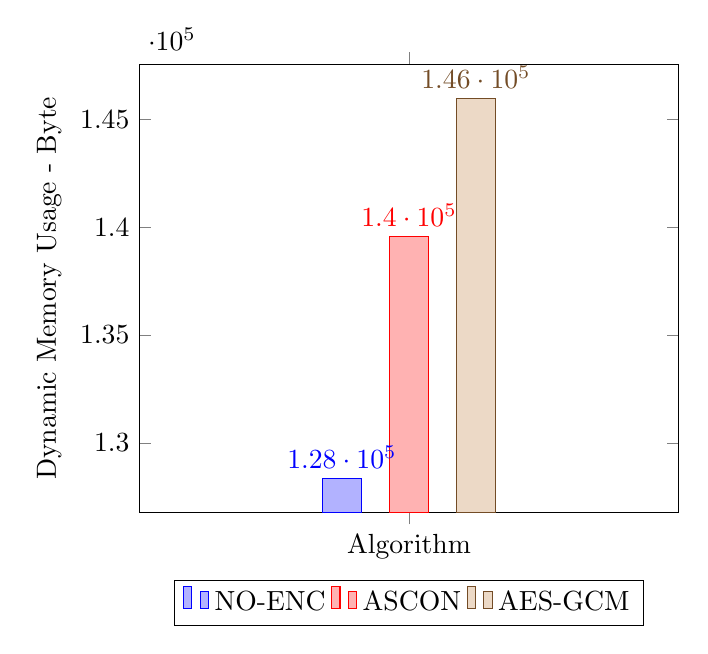
\begin{tikzpicture}
                    \begin{axis}[
                        ybar = 10pt,
                        enlargelimits=0.09,
                        legend style={at={(0.5,-0.15)},
                        anchor=north,legend columns=-1},
                        ylabel={Dynamic Memory Usage - Byte},
                        symbolic x coords={Algorithm},
                        xtick=data,
                        nodes near coords,
                        nodes near coords align={vertical},
                        bar width = 0.5cm,
                        ]
                        \addplot coordinates {(Algorithm,128356)};
                        \addplot coordinates {(Algorithm,139588)};
                        \addplot coordinates {(Algorithm,145972)};
                         
                        \legend{NO-ENC, ASCON, AES-GCM}
                    \end{axis}
                \end{tikzpicture}
            }
        \label{Fig:dynamic-memory}
    \end{subfigure}%
    \begin{subfigure}[c]{0.48\linewidth}
        \caption{The Additional Memory Overhead Introduced by the Algorithm.}
        \resizebox{\linewidth}{!}{
            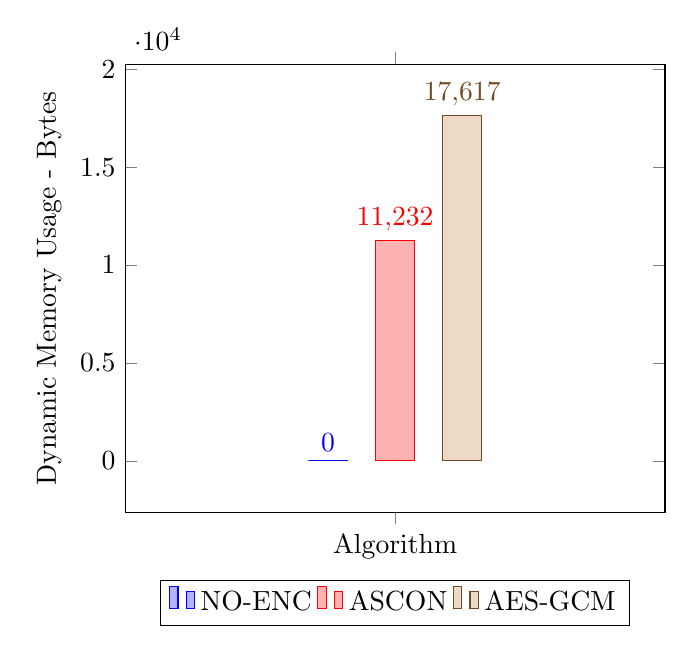
\begin{tikzpicture}
                \begin{axis}[
                    ybar = 10pt,
                    enlargelimits=0.15,
                    legend style={at={(0.5,-0.15)},
                    anchor=north,legend columns=-1},
                    ylabel={Dynamic Memory Usage - Bytes},
                    symbolic x coords={Algorithm},
                    xtick=data,
                    nodes near coords,
                    nodes near coords align={vertical},
                    bar width = 0.5cm,
                    ]
                    \addplot coordinates {(Algorithm,0)};
                    \addplot coordinates {(Algorithm, 11232)};
                    \addplot coordinates {(Algorithm, 17617)};
                    % \addplot coordinates {(Algorithm,2)};
                     
                    \legend{NO-ENC, ASCON, AES-GCM}
                \end{axis}
            \end{tikzpicture}
            }
    \label{Fig:memory-algo}
\end{subfigure}
\label{Fig:memory-impl-algo}
\end{figure}

\subsection{Power Consumption Measurement }